%!TEX program = xelatex
%!TEX root = ../all_beamer.tex

% ============================================================
% Beamer presentation: Chapter 4 – Probabilistic Learning
% Machine Learning Course – Giorgio Gambosi, Tor Vergata
% Modelled on the SLT Beamer style (ml-slt-beamer.pdf)
% ============================================================
%\documentclass[10pt,aspectratio=169]{beamer}
%
%% ---- Theme & colours ----------------------------------------
%\usetheme{Madrid}
%\usecolortheme{whale}
%\setbeamercolor{palette primary}{bg=structure.fg!80!black,fg=white}
%\setbeamercolor{frametitle}{bg=structure.fg!80!black,fg=white}
%\setbeamercolor{title}{bg=structure.fg!90!black,fg=white}
%\setbeamercolor{block title}{bg=structure.fg!70!black,fg=white}
%\setbeamercolor{block body}{bg=structure.fg!10!white}
%\setbeamercolor{block title alerted}{bg=red!70!black,fg=white}
%\setbeamercolor{block body alerted}{bg=red!10}
%\setbeamercolor{block title example}{bg=green!40!black,fg=white}
%\setbeamercolor{block body example}{bg=green!8}
%% !TEX root = all_beamer.tex
% ==============================================================================
% HEADER LATEX PER PRESENTAZIONI BEAMER
% Corso di Machine Learning - Giorgio Gambosi
% Università di Roma "Tor Vergata"
% ==============================================================================

% ------------------------------------------------------------------------------
% CLASSE DOCUMENTO E METADATI
% ------------------------------------------------------------------------------
\documentclass[aspectratio=169, 10pt]{beamer}

\subtitle{Course of Machine Learning}
\author{Giorgio Gambosi}
\institute[Tor Vergata]{Master's Degree in Computer Science\\University of Rome ``Tor Vergata''}
\date{A.Y. 2025--2026}

% ------------------------------------------------------------------------------
% PACCHETTI MATEMATICI
% ------------------------------------------------------------------------------
\usepackage{amsmath, amssymb, amsfonts, mathtools, amsthm}
\usepackage{bm}              % Simboli matematici in grassetto
\usepackage{upgreek}         % Lettere greche dritte
\usepackage{derivative}      % Gestione semplificata delle derivate

% ------------------------------------------------------------------------------
% PACCHETTI GRAFICI E VISUALIZZAZIONE
% ------------------------------------------------------------------------------
\usepackage{graphicx}        % Inclusione immagini
\usepackage{xcolor}          % Gestione colori
\usepackage{xkcdcolors}      % Colori aggiuntivi stile xkcd
\usepackage{microtype}       % Miglioramenti tipografici

% ------------------------------------------------------------------------------
% PACCHETTI PER TABELLE
% ------------------------------------------------------------------------------
\usepackage{booktabs}        % Tabelle professionali
\usepackage{array}           % Estensioni per tabelle
\usepackage{multirow}        % Celle multi-riga
\usepackage{multicol}        % Layout multi-colonna

% ------------------------------------------------------------------------------
% TIKZ E PGFPLOTS
% ------------------------------------------------------------------------------
\usepackage{tikz}
\usepackage{tikz-network}
\usepackage[customcolors]{hf-tikz}
\usepackage{pgfplots}
\pgfplotsset{compat=1.18}
\usepgfplotslibrary{fillbetween}

% Librerie TikZ
\usetikzlibrary{arrows, arrows.meta, decorations.pathmorphing, decorations.pathreplacing}
\usetikzlibrary{decorations.markings, snakes, positioning, backgrounds, fit, shadows}
\usetikzlibrary{automata, patterns, calc, intersections, through, shapes}
\usetikzlibrary{shapes.geometric, shapes.arrows, scopes, chains, matrix}

% ------------------------------------------------------------------------------
% ALTRI PACCHETTI
% ------------------------------------------------------------------------------
\usepackage[skins]{tcolorbox}  % Box colorati
\usepackage{subcaption}         % Sottocaption per figure
\usepackage{listings}           % Inclusione codice sorgente

% ------------------------------------------------------------------------------
% TEMA E STILE BEAMER
% ------------------------------------------------------------------------------
\usetheme{Madrid}
\usecolortheme{whale}
\useinnertheme{rounded}
\usefonttheme{professionalfonts}
\setbeamertemplate{navigation symbols}{}  % Rimuove simboli di navigazione

% ------------------------------------------------------------------------------
% DEFINIZIONE COLORI PERSONALIZZATI
% ------------------------------------------------------------------------------
% Colori principali del tema
\definecolor{MainBlue}{RGB}{31,56,100}      % Blu principale (header, titoli)
\definecolor{AccentBlue}{RGB}{70,130,180}   % Blu accento (blocchi)
\definecolor{AlertRed}{RGB}{160,30,30}      % Rosso per alert
\definecolor{ExGreen}{RGB}{30,120,60}       % Verde per esempi
\definecolor{BlockBg}{RGB}{220,232,246}     % Sfondo blocchi
\definecolor{torgray}{RGB}{220,225,235}     % Grigio Tor Vergata

% Colori alternativi (Tor Vergata style)
\definecolor{TvDark}{RGB}{30,50,80}         % Blu scuro header
\definecolor{TvMid}{RGB}{70,100,140}        % Blu medio blocchi
\definecolor{TvLight}{RGB}{210,220,235}     % Blu chiaro sfondi
\definecolor{TvAlert}{RGB}{160,30,30}       % Rosso alert
\definecolor{TvGreen}{RGB}{20,100,50}       % Verde esempi

% Colori supplementari
\definecolor{torred}{RGB}{153,0,0}
\definecolor{torcyan}{RGB}{0,112,192}
\definecolor{cerise}{HTML}{DA3A62}
\definecolor{teal}{HTML}{029386}
\definecolor{slateblue}{HTML}{5B5EA6}
\definecolor{orange}{HTML}{F97306}

% Colori per nodi TikZ
\definecolor{nodeblue}{RGB}{101,140,196}    % xkcd Faded Blue

% ------------------------------------------------------------------------------
% CONFIGURAZIONE COLORI BEAMER
% ------------------------------------------------------------------------------
\setbeamercolor{frametitle}{bg=MainBlue, fg=white}
\setbeamercolor{title}{bg=MainBlue, fg=white}
\setbeamercolor{structure}{fg=MainBlue}

% Blocchi standard
\setbeamercolor{block title}{bg=AccentBlue, fg=white}
\setbeamercolor{block body}{bg=BlockBg}

% Blocchi alert
\setbeamercolor{block title alerted}{bg=AlertRed, fg=white}
\setbeamercolor{block body alerted}{bg=red!8}

% Blocchi esempio
\setbeamercolor{block title example}{bg=ExGreen, fg=white}
\setbeamercolor{block body example}{bg=green!7}

% ------------------------------------------------------------------------------
% CONFIGURAZIONE FONT BEAMER
% ------------------------------------------------------------------------------
\setbeamerfont{frametitle}{size=\normalsize,series=\bfseries}
\setbeamerfont{block title}{size=\small,series=\bfseries}

% ------------------------------------------------------------------------------
% STILI TIKZ PERSONALIZZATI
% ------------------------------------------------------------------------------
\tikzset{
  >=latex,  % Frecce stile LaTeX di default
  % Nodi per reti neurali
  node/.style={thick,circle,draw=myblue,minimum size=22,inner sep=0.5,outer sep=0.6},
  node in/.style={node,green!20!black,draw=mygreen!30!black,fill=mygreen!25},
  node hidden/.style={node,blue!20!black,draw=myblue!30!black,fill=myblue!20},
  node convol/.style={node,orange!20!black,draw=myorange!30!black,fill=myorange!20},
  node out/.style={node,red!20!black,draw=myred!30!black,fill=myred!20},
  % Connessioni
  connect/.style={thick,mydarkblue},
  connect arrow/.style={-{Latex[length=4,width=3.5]},thick,mydarkblue,shorten <=0.5,shorten >=1},
  % Stili numerati per facile mappatura
  node 1/.style={node in},
  node 2/.style={node hidden},
  node 3/.style={node out}
}

% ------------------------------------------------------------------------------
% AMBIENTI TEOREMI
% ------------------------------------------------------------------------------
\setbeamertemplate{theorems}[numbered]
\newtheorem{mytheorem}{Theorem}
\newtheorem{mydefinition}{Definition}

% ------------------------------------------------------------------------------
% CONFIGURAZIONE LISTINGS (CODICE)
% ------------------------------------------------------------------------------
\lstset{
  language=Python,
  basicstyle=\ttfamily\tiny,
  keywordstyle=\color{MainBlue}\bfseries,
  commentstyle=\color{gray},
  frame=single,
  breaklines=true,
}

% ==============================================================================
% MACRO MATEMATICHE PERSONALIZZATE
% ==============================================================================

% ------------------------------------------------------------------------------
% SPAZI CALLIGRAFICI (Calligraphic spaces)
% ------------------------------------------------------------------------------
\providecommand{\calX}{\mathcal{X}}         % Spazio input
\providecommand{\calY}{\mathcal{Y}}         % Spazio output
\providecommand{\calH}{\mathcal{H}}         % Spazio ipotesi
\providecommand{\calT}{\mathcal{T}}         % Training set
\providecommand{\calA}{\mathcal{A}}         % Algoritmo
\providecommand{\calR}{\mathcal{R}}         % Rischio
\providecommand{\calF}{\mathcal{F}}         % Famiglia di funzioni
\providecommand{\calL}{\mathcal{L}}         % Loss function

% Alias per compatibilità
\providecommand{\Rr}{\mathcal{R}}
\providecommand{\Tr}{\mathcal{T}}
\providecommand{\Hr}{\mathcal{H}}

% ------------------------------------------------------------------------------
% RISCHIO E PROBABILITÀ
% ------------------------------------------------------------------------------
\providecommand{\barR}{\overline{\mathcal{R}}}  % Rischio empirico
\providecommand{\EmpR}{\overline{\mathcal{R}}}  % Rischio empirico (alias)
\providecommand{\Rbar}{\overline{\mathcal{R}}}  % Rischio empirico (alias)
\providecommand{\pM}{p_M}                       % Probabilità modello
\providecommand{\pC}{p_C}                       % Probabilità corretta
\providecommand{\Prob}[2]{\mathbb{P}_{#1}\!\left[#2\right]}  % Probabilità

% ------------------------------------------------------------------------------
% FUNZIONI INDICATRICI
% ------------------------------------------------------------------------------
\providecommand{\indicator}[1]{\mathbf{1}\!\left[#1\right]}  % Funzione indicatrice
\providecommand{\ind}[1]{\mathbf{1}[#1]}                      % Versione breve

% ------------------------------------------------------------------------------
% OPERATORI MATEMATICI
% ------------------------------------------------------------------------------
\providecommand{\argmax}{\operatorname*{arg\,max}}  % Argomento del massimo
\providecommand{\argmin}{\operatorname*{arg\,min}}  % Argomento del minimo
\providecommand{\vcd}[1]{\operatorname{VCdim}(#1)} % VC dimension
\providecommand{\defeq}{\stackrel{\text{def}}{=}}  % Definito come

% ------------------------------------------------------------------------------
% VETTORI E MATRICI (Bold Math)
% ------------------------------------------------------------------------------
% Vettori minuscoli
\providecommand{\bx}{\mathbf{x}}            % Vettore x
\providecommand{\bz}{\mathbf{z}}            % Vettore z
\providecommand{\bw}{\mathbf{w}}            % Vettore peso
\providecommand{\btt}{\mathbf{t}}           % Vettore target
\providecommand{\wvec}{\mathbf{w}}          % Vettore peso (alias)
\providecommand{\bth}{\boldsymbol{\theta}}  % Parametro theta

% Matrici maiuscole
\providecommand{\bX}{\mathbf{X}}            % Matrice dati
\providecommand{\bZ}{\mathbf{Z}}            % Matrice Z
\providecommand{\Xmat}{\mathbf{X}}          % Matrice dati (alias)
\providecommand{\Hmat}{\mathbf{H}}          % Matrice H
\providecommand{\Smat}{\mathbf{S}}          % Matrice scatter generica
\providecommand{\bS}{\mathbf{S}}            % Matrice scatter
\providecommand{\Ii}{\mathbf{I}}            % Matrice identità
\providecommand{\bZero}{\mathbf{0}}         % Vettore zero
\providecommand{\bPsi}{\boldsymbol{\Psi}}   % Matrice Psi

% Medie (overline)
\providecommand{\ox}{\overline{\mathbf{x}}} % Media vettore x
\providecommand{\ow}{\overline{\mathbf{w}}} % Media vettore w
\providecommand{\oX}{\overline{\mathbf{X}}} % Media matrice X

% Matrici scatter specifiche (analisi discriminante)
\providecommand{\SW}{\mathbf{S}_W}          % Within-class scatter
\providecommand{\SB}{\mathbf{S}_B}          % Between-class scatter
\providecommand{\ST}{\mathbf{S}_T}          % Total scatter
\providecommand{\GX}{G_{\mathbf{X}}}        % Matrice Gram

% ------------------------------------------------------------------------------
% COMANDI DI FORMATTAZIONE TESTO
% ------------------------------------------------------------------------------
\providecommand{\term}[1]{\textbf{\color{accent}#1}}        % Termine importante
\providecommand{\halert}[1]{{\color{AlertRed}\textbf{#1}}}  % Alert rosso
\providecommand{\mlalert}[1]{{\color{AccentBlue}\textbf{#1}}}  % Alert blu
\providecommand{\mlemph}[1]{{\color{MainBlue}\textit{#1}}}  % Enfasi blu

% ==============================================================================
% FINE HEADER
% ==============================================================================

\newcommand{\blankpage}{
\clearpage
\thispagestyle{empty}
\null
\clearpage
}

% ---- Packages -----------------------------------------------
%\usepackage{amsmath,amssymb,bm}
%\usepackage{mathtools}
%\usepackage{booktabs}
%\usepackage{xcolor}
%\usepackage{tikz}
%\usetikzlibrary{arrows.meta,shapes,positioning,fit,calc}
%\usepackage{graphicx}

% ---- Macros -------------------------------------------------


%\DeclareMathOperator*{\argmax}{arg\,max}
%\DeclareMathOperator*{\argmin}{arg\,min}

% ---- Navigation dots style ----------------------------------
%\setbeamertemplate{navigation symbols}{}
%\setbeamertemplate{footline}[frame number]

% ---- Title page info ----------------------------------------
\title[Probabilistic Learning]{Probabilistic Learning}
%\subtitle{Course of Machine Learning}
%\author{Giorgio Gambosi}
%\institute{Master's Degree in Computer Science\\University of Rome ``Tor Vergata''}
%\date{A.Y. 2025--2026}

% =============================================================
%\begin{document}

\begin{frame}
  \titlepage
\end{frame}

% ---- OUTLINE ------------------------------------------------
\begin{frame}{Outline}
  \tableofcontents
\end{frame}

% =============================================================
\section{Probabilistic Framework}
% =============================================================

\subsection{The Probabilistic Setting}

\begin{frame}{Probabilistic Framework}{The Supervised Learning Setting}
  \begin{block}{Data Generating Process}
    Observed data are generated by random sampling:
    \begin{itemize}
      \item Features $\x \in \mathcal{X}$ drawn from marginal distribution $p_M(\x)$
      \item Targets $t \in \mathcal{Y}$ drawn from conditional distribution $p_C(t|\x)$
    \end{itemize}
  \end{block}

  \bigskip
  \textbf{Goal}: from training set $\mathcal{T}$, derive an approximation $p^*(t|\x) \approx p_C(t|\x)$.

  \begin{itemize}
    \item A \textbf{probabilistic predictor} returns $p^*(t|\x)$, not a single value.
    \item A \textbf{decision strategy} is applied separately to produce the final prediction:
    \[
      h(\x) = \argmax_{t \in \mathcal{Y}} p^*(t|\x)
    \]
    \item Different decision strategies can accommodate asymmetric costs.
  \end{itemize}
\end{frame}

\begin{frame}{Probabilistic Framework}{Why Probabilistic Models?}
  \begin{columns}
    \begin{column}{0.48\textwidth}
      \begin{block}{Functional Predictors}
        \begin{itemize}
          \item Return a single prediction $h(\x)$
          \item Optimize empirical risk directly
          \item No explicit uncertainty quantification
        \end{itemize}
      \end{block}
    \end{column}
    \begin{column}{0.48\textwidth}
      \begin{alertblock}{Probabilistic Predictors}
        \begin{itemize}
          \item Return a full distribution $p^*(t|\x)$
          \item Capture uncertainty explicitly
          \item Support principled decision-making under cost asymmetries
        \end{itemize}
      \end{alertblock}
    \end{column}
  \end{columns}

  \bigskip
  \begin{exampleblock}{Key Insight}
    The probabilistic approach separates \textbf{inference} (learning $p^*$) from \textbf{decision} (choosing an action given $p^*$). This modularity is powerful and principled.
  \end{exampleblock}
\end{frame}

% =============================================================
\section{Decision Theory}
% =============================================================

\subsection{Classification Decisions}

\begin{frame}{Decision Theory}{Decision Regions and Boundaries}
  \begin{block}{Setup}
    Partition input space $\mathcal{X}$ into $K$ disjoint \textbf{decision regions} $\mathcal{R}_1, \ldots, \mathcal{R}_K$.
    \begin{itemize}
      \item $\x \in \mathcal{R}_k \Rightarrow$ assigned to class $\mathcal{C}_k$
      \item Boundaries between regions are \textbf{decision boundaries}
    \end{itemize}
  \end{block}

  \textbf{Optimal rule for binary classification} — maximize probability of being correct:
  \[
    \hat{p}(\x) = \int_{\mathcal{R}_0} p(\x,\mathcal{C}_0)\,d\x + \int_{\mathcal{R}_1} p(\x,\mathcal{C}_1)\,d\x
  \]
  
  \begin{itemize}
    \item Assign $\x$ to class with highest \textbf{posterior probability}:
    \[
      h(\x) = \argmax_{k} \; p(\mathcal{C}_k|\x)
    \]
    \item This extends naturally to $K > 2$ classes.
  \end{itemize}
\end{frame}

\begin{frame}{Decision Theory}{Multi-class Optimal Classifier}
  For $K$ classes, the probability of correct classification is:
  \[
    \hat{p}(\x) = \sum_{i=0}^{K-1} \int_{\mathcal{R}_i} p(\x, \mathcal{C}_i)\,d\x
  \]

  \begin{block}{Optimal Decision Rule}
    \[
      h(\x) = \argmax_{0 \le i \le K-1} \; p(\mathcal{C}_i|\x)
    \]
    Choose the class with the \textbf{maximum posterior probability}.
  \end{block}

  \begin{itemize}
    \item This is the \textbf{Bayes optimal classifier} — achieves minimum 0/1 loss in expectation.
    \item Requires knowledge of the full posterior $p(\mathcal{C}_k|\x)$ — rarely available in practice.
    \item In practice, we \emph{approximate} this posterior from training data.
  \end{itemize}
\end{frame}

\subsection{Incorporating Misclassification Costs}

\begin{frame}{Decision Theory}{The Loss Matrix}
  \begin{block}{Loss Matrix $L_{ij}$}
    $L_{ij}$ = cost of classifying an item as $\mathcal{C}_j$ when it truly belongs to $\mathcal{C}_i$.
  \end{block}

  \textbf{Expected cost (risk)} of decision regions:
  \[
    \mathbb{E}[L] = \sum_j \int_{\mathcal{R}_j} \left[\sum_i L_{ij}\,p(\mathcal{C}_i|\x)\right] p(\x)\,d\x
  \]

  \textbf{Optimal assignment}: for each $\x$, choose the class $k$ minimising the \textbf{conditional risk}:
  \[
    j = \argmin_k \sum_i L_{ik}\,p(\mathcal{C}_i|\x)
  \]

  \begin{itemize}
    \item When $L_{ij} = 1 - \delta_{ij}$ (equal costs), this reduces to the max-posterior rule.
    \item Asymmetric costs shift the decision threshold.
  \end{itemize}
\end{frame}

\begin{frame}{Decision Theory}{Binary Classification with Costs}
  Assign $\x$ to $\mathcal{R}_0$ if the cost for $\mathcal{C}_0$ is lower:
  \[
    (L_{10} - L_{00})\,p(\mathcal{C}_0|\x) > (L_{01} - L_{11})\,p(\mathcal{C}_1|\x)
  \]

  Define threshold $\theta = \dfrac{L_{01}-L_{11}}{L_{10}+L_{01}-L_{00}-L_{11}}$.

  \begin{block}{Decision Rule}
    Assign $\x$ to $\mathcal{C}_0$ if $p(\mathcal{C}_0|\x) > \theta$.
  \end{block}

  \begin{exampleblock}{Medical Diagnosis Example}
    $\mathcal{C}_0 = \text{Sick}$, $\mathcal{C}_1 = \text{Healthy}$, $L = \begin{pmatrix}0 & 100\\ 1 & 0\end{pmatrix}$.\\
    Missing a sick patient (cost 100) is 100$\times$ more costly than a false alarm.\\[4pt]
    Assign "Healthy" only if $p(\mathcal{C}_1|\x) > \dfrac{100}{101} \approx 0.99$.
  \end{exampleblock}
\end{frame}

\subsection{The Reject Option}

\begin{frame}{Decision Theory}{The Reject Option}
  \begin{block}{Motivation}
    When uncertainty is very high, the most rational action may be to \textbf{refuse to predict}.
  \end{block}

  Introduce a \textbf{rejection region}: 
  \[
    h(\x) = \begin{cases}
      0 & \text{if } p(\mathcal{C}_0|\x) > \theta' \\
      1 & \text{if } p(\mathcal{C}_0|\x) < 1-\theta'' \\
      \text{undefined} & \text{otherwise}
    \end{cases}
  \]

  \begin{itemize}
    \item $\theta'$ and $1-\theta''$ are derived by scaling costs with a safety margin $(1-\varepsilon)$.
    \item The gap between $\theta'$ and $1-\theta''$ is the \textbf{rejection region}.
    \item Higher misclassification costs $\Rightarrow$ wider rejection region.
    \item Common in medical diagnosis, safety-critical systems, credit scoring.
  \end{itemize}
\end{frame}

\subsection{Decision Theory for Regression}

\begin{frame}{Decision Theory}{Regression: Squared Loss Optimum}
  For continuous targets, the most common loss is the \textbf{squared loss}:
  \[
    \mathbb{E}[L] = \iint (h(\x) - t)^2\,p(\x,t)\,d\x\,dt
  \]

  \textbf{Decomposition}:
  \[
    (h(\x) - t)^2 = \underbrace{(h(\x)-\mathbb{E}[t|\x])^2}_{\text{controllable}} + \underbrace{(\mathbb{E}[t|\x]-t)^2}_{\text{irreducible noise}} + \text{cross term} = 0
  \]

  \begin{block}{Optimal Regression Predictor}
    The first term vanishes when:
    \[
      h^*(\x) = \mathbb{E}[t|\x] = \int t\,p(t|\x)\,dt
    \]
    The optimal prediction is the \textbf{conditional mean} of the target.
  \end{block}
\end{frame}

% =============================================================
\section{Approximating the Conditional Distribution}
% =============================================================

\subsection{Generative vs.\ Discriminative Models}

\begin{frame}{Approximating $p_C(\x, t)$}{The Core Challenge}
  \begin{alertblock}{Problem}
    Decision theory assumes $p_C(t|\x)$ is \emph{known}. In practice, we only have a finite training set $\mathcal{T}$.
  \end{alertblock}

  \textbf{Goal}: learn $p^*(t|\x) \approx p_C(t|\x)$ from $\mathcal{T}$.

  \bigskip
  \begin{columns}
    \begin{column}{0.47\textwidth}
      \begin{block}{Generative Models}
        \begin{itemize}
          \item Model class-conditional densities $p(\x|\mathcal{C}_k)$ and priors $p(\mathcal{C}_k)$
          \item Apply Bayes' rule to get posterior
          \item Example: Naive Bayes, Gaussian mixtures
        \end{itemize}
      \end{block}
    \end{column}
    \begin{column}{0.47\textwidth}
      \begin{block}{Discriminative Models}
        \begin{itemize}
          \item Directly estimate $p(\mathcal{C}_k|\x)$
          \item No modelling of input distribution
          \item Example: Logistic Regression, Neural Nets
        \end{itemize}
      \end{block}
    \end{column}
  \end{columns}
\end{frame}

\begin{frame}{Approximating $p_C(\x, t)$}{Generative Approach: Bayes' Rule}
  \begin{block}{Bayes' Rule for Classification}
    \[
      p(\mathcal{C}_k|\x) = \frac{p(\x|\mathcal{C}_k)\,p(\mathcal{C}_k)}{p(\x)} = \frac{p(\x|\mathcal{C}_k)\,p(\mathcal{C}_k)}{\sum_j p(\x|\mathcal{C}_j)\,p(\mathcal{C}_j)}
    \]
  \end{block}

  \begin{itemize}
    \item $p(\x|\mathcal{C}_k)$ — class-conditional density (requires generative model)
    \item $p(\mathcal{C}_k)$ — prior class probability
    \item $p(\x)$ — normalizing constant (marginal)
    \item Only the product $p(\x|\mathcal{C}_k)\,p(\mathcal{C}_k)$ is needed for comparison
  \end{itemize}

  \begin{exampleblock}{Advantage}
    Can handle outlier detection, synthesis, and missing data naturally.
  \end{exampleblock}
\end{frame}

\begin{frame}{Approximating $p_C(\x, t)$}{Three-Step Learning Procedure}
  \begin{enumerate}
    \item[\textbf{1.}] \textbf{Model Selection}: Define a hypothesis space $\mathcal{P}$ — a class of candidate distributions.
    \item[\textbf{2.}] \textbf{Inference}: Select the ``best'' $p^* \in \mathcal{P}$ using training data $\mathcal{T}$ and quality measure $q$.
    \item[\textbf{3.}] \textbf{Prediction}: For new $\x$, use $p^*(t|\x)$ to assign probabilities and make decisions.
  \end{enumerate}

  \bigskip
  \begin{center}
  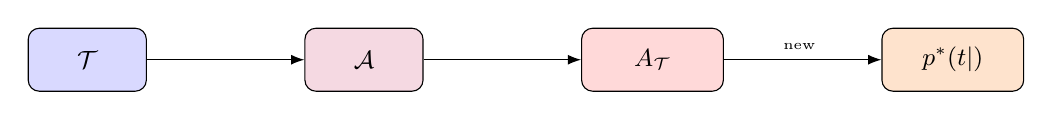
\begin{tikzpicture}[node distance=2cm, >=Latex, font=\small]
    \node[draw, fill=blue!15, rounded corners, minimum width=1.5cm, minimum height=0.8cm] (T) {$\mathcal{T}$};
    \node[draw, fill=purple!15, rounded corners, minimum width=1.5cm, minimum height=0.8cm, right=of T] (A) {$\mathcal{A}$};
    \node[draw, fill=red!15, rounded corners, minimum width=1.8cm, minimum height=0.8cm, right=of A] (AT) {$A_{\mathcal{T}}$};
    \node[draw, fill=orange!20, rounded corners, minimum width=1.8cm, minimum height=0.8cm, right=of AT] (p) {$p^*(t|\x)$};
    \draw[->] (T) -- (A);
    \draw[->] (A) -- (AT);
    \draw[->] (AT) -- node[above,font=\tiny]{new $\x$} (p);
  \end{tikzpicture}
  \end{center}
\end{frame}

\subsection{Parametric Models}

\begin{frame}{Parametric Distributions}{Logistic Regression Example}
  \begin{block}{Parametric Approach}
    Assume distributions share a mathematical structure governed by parameters $\w$. Learning = finding the best $\w$.
  \end{block}

  \begin{exampleblock}{Binary Classification: Logistic Regression}
    Target $t \in \{0,1\}$ follows a Bernoulli distribution:
    \[
      p(t|\x,\w) = \pi(\x)^t\,(1-\pi(\x))^{1-t}
    \]
    where $\pi(\x) = p(t=1|\x)$ is modelled via the \textbf{logistic sigmoid}:
    \[
      \pi(\x) = \sigma(\w^T\x) = \frac{1}{1 + e^{-(\sum_i w_i x_i + w_0)}}
    \]
    \begin{itemize}
      \item Squashes linear output to $[0,1]$ — interpretable as probability.
      \item Linear decision boundary in feature space.
    \end{itemize}
  \end{exampleblock}
\end{frame}

% =============================================================
\section{Maximum Likelihood Estimation}
% =============================================================

\subsection{Likelihood}

\begin{frame}{Maximum Likelihood Estimation}{The Likelihood Function}
  \begin{block}{Definition}
    The \textbf{likelihood} of parameters $\Vtheta$ given data $\mathcal{T}$ is:
    \[
      L(\Vtheta|\mathcal{T}) = p(\mathcal{T}|\Vtheta)
    \]
    \begin{itemize}
      \item $p(\mathcal{T}|\Vtheta)$: probability of the data (data varies, $\Vtheta$ fixed)
      \item $L(\Vtheta|\mathcal{T})$: likelihood of parameters (data fixed, $\Vtheta$ varies)
      \item Same mathematical form — different conceptual roles
    \end{itemize}
  \end{block}

  \textbf{i.i.d.\ factorization}:
  \begin{itemize}
    \item \textit{Density estimation}: $L(\Vtheta|\mathcal{T}) = \prod_{i=1}^n p(\x_i|\Vtheta)$
    \item \textit{Supervised learning}: $L(\Vtheta|\mathcal{T}) \propto \prod_{i=1}^n p(t_i|\x_i,\Vtheta)$
  \end{itemize}
\end{frame}

\begin{frame}{Maximum Likelihood Estimation}{MLE Optimization}
  \begin{block}{Maximum Likelihood Principle}
    \[
      \Vtheta^*_{ML} = \argmax_{\Vtheta} L(\Vtheta|\mathcal{T})
    \]
    Find the parameters that make the observed data most probable.
  \end{block}

  \textbf{Log-likelihood} (numerically stable, same optima):
  \[
    l(\Vtheta|\mathcal{T}) = \ln L(\Vtheta|\mathcal{T}) \qquad \Vtheta^*_{ML} = \argmax_{\Vtheta}\; l(\Vtheta|\mathcal{T})
  \]

  \textbf{Optimization procedure}: set gradient to zero (necessary condition):
  \[
    \nabla l(\Vtheta|\mathcal{T}) = \Zero
  \]

  \begin{itemize}
    \item Stationary point — verify with Hessian (second derivatives).
    \item May be a local maximum, minimum, or saddle point.
  \end{itemize}
\end{frame}

\subsection{MLE Examples}

\begin{frame}{MLE}{Example: Bernoulli Trials}
  \begin{exampleblock}{Coin Flips}
    $n$ binary events; $n_1$ successes, $n_0$ failures.

    Likelihood:
    \[
      L(\phi|\X) = \phi^{n_1}(1-\phi)^{n_0}
    \]
    Log-likelihood:
    \[
      l(\phi|\X) = n_1 \ln\phi + n_0\ln(1-\phi)
    \]
    Setting derivative to zero:
    \[
      \frac{n_1}{\phi} - \frac{n_0}{1-\phi} = 0 \implies \phi^*_{ML} = \frac{n_1}{n_1+n_0} = \frac{n_1}{n}
    \]
    \textbf{Result}: MLE = observed sample frequency (intuitive frequentist result).
  \end{exampleblock}
\end{frame}

\begin{frame}{MLE}{Example: Linear Regression with Gaussian Noise}
  Model: $p(t|\x,\w,\sigma^2) = \mathcal{N}(\w^T\x + w_0,\,\beta^{-1})$, where $\beta$ is precision.

  Log-likelihood:
  \[
    l(\t|\X,\w,w_0,\beta) = -\frac{\beta}{2}\sum_{i=1}^n(\w^T\x_i+w_0-t_i)^2 + \frac{n}{2}\ln\beta - \frac{n}{2}\ln(2\pi)
  \]

  \begin{block}{MLE for Regression Coefficients}
    Setting gradients w.r.t.\ $\w, w_0$ to zero yields a linear system:
    \[
      \sum_{i=1}^n(\w^T\x_i+w_0-t_i)\,x_{ik} = 0 \quad k=1,\ldots,d; \qquad \sum_{i=1}^n(\w^T\x_i+w_0-t_i) = 0
    \]
  \end{block}
  \begin{block}{MLE for Precision $\beta$}
    \[
      \beta_{ML} = \left(\frac{1}{n}\sum_{i=1}^n(\w^T\x_i+w_0-t_i)^2\right)^{-1}
    \]
    Inverse of the mean squared error.
  \end{block}
\end{frame}

\begin{frame}{MLE}{Connection to Empirical Risk Minimisation}
  \begin{alertblock}{Key Insight}
    Maximizing log-likelihood under Gaussian noise is \emph{equivalent} to minimising the sum of squared errors (L2 loss).
  \end{alertblock}

  \begin{itemize}
    \item MLE under Bernoulli likelihood $\equiv$ minimising cross-entropy loss.
    \item The choice of \textbf{noise model} determines the \textbf{loss function}.
    \item Probabilistic framework provides a principled derivation of loss functions.
  \end{itemize}

  \begin{block}{Predictions from MLE}
    After finding $\Vtheta^*_{ML}$:
    \[
      p(\x|\X) \approx p(\x|\Vtheta^*_{ML}), \qquad p(t|\x,\X,\t) \approx p(t|\x,\Vtheta^*_{ML})
    \]
  \end{block}
\end{frame}

\subsection{Overfitting and MAP}

\begin{frame}{Overfitting and MAP}{Problem with Pure MLE}
  \begin{alertblock}{Overfitting}
    MLE may ``memorize'' the noise in $\mathcal{T}$, leading to poor generalization on new data.
  \end{alertblock}

  \textbf{Remedy}: add a \textbf{penalty function} $P(\Vtheta)$ to the log-likelihood:
  \[
    C(\Vtheta|\X) = l(\Vtheta|\X) - P(\Vtheta)
  \]
  Common choice: $L_2$ regularization (weight decay):
  \[
    P(\Vtheta) = \frac{\gamma}{2}\|\Vtheta\|^2
  \]

  \begin{itemize}
    \item Penalizes large parameter values.
    \item Controlled by hyperparameter $\gamma > 0$.
    \item Has a deep Bayesian interpretation (MAP estimation).
  \end{itemize}
\end{frame}

\begin{frame}{Overfitting and MAP}{Maximum A Posteriori (MAP)}
  \begin{block}{Bayesian Interpretation of Regularization}
    Treat $\Vtheta$ as a random variable with prior $p(\Vtheta)$. By Bayes' theorem:
    \[
      p(\Vtheta|\mathcal{T}) \propto L(\Vtheta|\mathcal{T})\,p(\Vtheta)
    \]
    The \textbf{MAP estimate} maximizes the posterior:
    \[
      \Vtheta^*_{MAP} = \argmax_{\Vtheta}\left(\ln L(\Vtheta|\mathcal{T}) + \ln p(\Vtheta)\right)
    \]
  \end{block}

  With Gaussian prior $p(\Vtheta) \sim \mathcal{N}(\Zero,\sigma^2\mathbf{I})$:
  \[
    \Vtheta^*_{MAP} = \argmax_{\Vtheta}\left(l(\Vtheta|\mathcal{T}) - \frac{\|\Vtheta\|^2}{2\sigma^2}\right)
  \]

  \begin{exampleblock}{Result}
    MAP with Gaussian prior $\equiv$ $L_2$-regularized MLE, with $\gamma = 1/\sigma^2$.\\
    \textbf{Regularization = encoded prior belief that parameters should be small.}
  \end{exampleblock}
\end{frame}

\begin{frame}{MAP}{Example: Bernoulli with Beta Prior}
  \begin{exampleblock}{Beta-Bernoulli Conjugate Pair}
    Prior: $p(\phi|\alpha,\beta) = \mathrm{Beta}(\phi|\alpha,\beta) \propto \phi^{\alpha-1}(1-\phi)^{\beta-1}$

    Log-posterior: $l(\phi|\X) + \ln p(\phi|\alpha,\beta) = n_1\ln\phi + n_0\ln(1-\phi) + (\alpha-1)\ln\phi + (\beta-1)\ln(1-\phi)$

    Setting derivative to zero:
    \[
      \phi^*_{MAP} = \frac{n_1 + \alpha - 1}{n + \alpha + \beta - 2}
    \]

    \begin{itemize}
      \item $\alpha, \beta$ act as \textbf{pseudo-counts} from prior experience.
      \item Prevents estimates from being 0 or 1 with scarce data.
      \item Solves the ``\textbf{black swan problem}'': never seeing X doesn't mean $p(X)=0$.
    \end{itemize}
  \end{exampleblock}
\end{frame}

% =============================================================
\section{Full Bayesian Inference}
% =============================================================

\subsection{Beyond MAP}

\begin{frame}{Full Bayesian Inference}{Limitations of MAP}
  \begin{block}{Posterior Distribution}
    \[
      p(\Vtheta|\X) = \frac{p(\X|\Vtheta)\,p(\Vtheta)}{\int p(\X|\Vtheta)\,d\Vtheta}
    \]
  \end{block}

  MAP computes only the \textbf{mode} of the posterior — this can be misleading if:
  \begin{itemize}
    \item The posterior is \textbf{skewed} (mode $\ne$ mean)
    \item The posterior is \textbf{multimodal} (multiple equally valid parameter values)
  \end{itemize}

  \begin{center}
  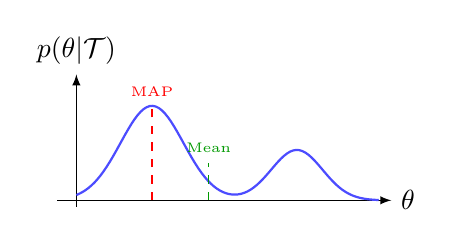
\begin{tikzpicture}[scale=0.8]
    \draw[->] (-0.3,0) -- (5,0) node[right] {$\theta$};
    \draw[->] (0,-0.1) -- (0,2) node[above] {$p(\theta|\mathcal{T})$};
    \draw[blue!70, thick, domain=0:4.8, samples=100]
      plot (\x, {1.5*exp(-2*(\x-1.2)^2) + 0.8*exp(-3*(\x-3.5)^2)});
    \draw[red, dashed] (1.2,0) -- (1.2,1.5) node[above,red,font=\tiny]{MAP};
    \draw[green!60!black, dashed] (2.1,0) -- (2.1,0.6) node[above,green!60!black,font=\tiny]{Mean};
  \end{tikzpicture}
  \end{center}
  \small\textit{Bimodal posterior: MAP gives the left peak, but the mean lies in a low-density region.}
\end{frame}

\begin{frame}{Full Bayesian Inference}{Posterior Mean and Predictive Distribution}
  \begin{block}{Full Bayesian Approach}
    Use the \textbf{entire posterior distribution} $p(\Vtheta|\X)$.

    \textbf{Posterior mean}:
    \[
      \Vtheta^* = \mathbb{E}[\Vtheta|\X] = \int \Vtheta\, p(\Vtheta|\X)\,d\Vtheta
    \]
  \end{block}

  \begin{block}{Predictive Distribution}
    For new $\x$, average over all parameter settings:
    \[
      p(\x_\text{new}|\X) = \int p(\x_\text{new}|\Vtheta)\,p(\Vtheta|\X)\,d\Vtheta
    \]
    \[
      p(t|\x_\text{new},\X,\t) = \int p(t|\x_\text{new},\Vtheta)\,p(\Vtheta|\X,\t)\,d\Vtheta
    \]
  \end{block}

  \begin{itemize}
    \item Integrates out all parameter uncertainty — more robust predictions.
    \item Computationally expensive (often requires approximations).
  \end{itemize}
\end{frame}

\begin{frame}{Full Bayesian Inference}{Example: Beta-Bernoulli Update}
  \begin{exampleblock}{Conjugate Bayesian Update}
    Prior: $p(\phi|\alpha,\beta) = \mathrm{Beta}(\phi|\alpha,\beta)$

    Likelihood of $n$ i.i.d.\ binary observations ($n_1$ ones, $n_0$ zeros):
    \[
      p(\X|\phi) = \phi^{n_1}(1-\phi)^{n_0}
    \]

    Posterior (by conjugacy):
    \[
      p(\phi|\X,\alpha,\beta) = \mathrm{Beta}(\phi|\alpha+n_1,\;\beta+n_0)
    \]

    \begin{itemize}
      \item $\alpha \to \alpha + n_1$: prior successes increase with observed successes.
      \item $\beta \to \beta + n_0$: prior failures increase with observed failures.
      \item The Beta family is \textbf{conjugate} to the Bernoulli likelihood.
    \end{itemize}
  \end{exampleblock}
\end{frame}

% =============================================================
\section{Model Selection}
% =============================================================

\subsection{The Model Selection Problem}

\begin{frame}{Model Selection}{The Fundamental Dilemma}
  \begin{block}{Model Selection Problem}
    Before estimating parameters $\Vtheta$, we must choose the \textbf{model structure} itself:
    \begin{itemize}
      \item Functional form (linear, polynomial, neural network?)
      \item Number of features / basis functions
      \item Values of hyperparameters
    \end{itemize}
  \end{block}

  \begin{columns}
    \begin{column}{0.47\textwidth}
      \begin{alertblock}{Underfitting (Bias)}
        Model too simple — fails to capture the true signal.
        \begin{itemize}
          \item High training error
          \item High test error
        \end{itemize}
      \end{alertblock}
    \end{column}
    \begin{column}{0.47\textwidth}
      \begin{alertblock}{Overfitting (Variance)}
        Model too complex — captures noise in $\mathcal{T}$.
        \begin{itemize}
          \item Low training error
          \item High test error
        \end{itemize}
      \end{alertblock}
    \end{column}
  \end{columns}

  \bigskip
  \textbf{Goal}: find the model whose \emph{best instantiation} generalizes to unseen data.
\end{frame}

\subsection{Validation Strategies}

\begin{frame}{Model Selection}{Test Set Validation}
  \begin{block}{Holdout / Test Set Method}
    Partition $\mathcal{T}$ into two disjoint sets:
    \begin{itemize}
      \item \textbf{Training set}: learn parameters $\Vtheta$
      \item \textbf{Test set}: held out — provides unbiased performance estimate
    \end{itemize}
  \end{block}

  \begin{itemize}
    \item Computationally efficient and reliable for \textbf{large} datasets.
    \item For \textbf{small} datasets: too few points for robust fitting \emph{and} significant evaluation.
    \item Test set must be used \textbf{only once} — otherwise data leakage.
  \end{itemize}

  \begin{exampleblock}{Typical split}
    70/30 or 80/20 for training/test. For model selection + final evaluation, use 60/20/20 (train/validation/test).
  \end{exampleblock}
\end{frame}

\begin{frame}{Model Selection}{$K$-Fold Cross-Validation}
  \begin{block}{$K$-Fold Cross-Validation}
    \begin{enumerate}
      \item Partition $\mathcal{T}$ into $K$ equal-sized subsets (folds).
      \item Repeat $K$ times: use one fold as test set, union of remaining $K-1$ as training.
      \item Report the \textbf{average} performance across all $K$ iterations.
    \end{enumerate}
  \end{block}

  \begin{center}
  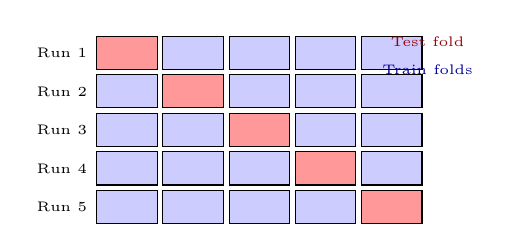
\begin{tikzpicture}[scale=0.7]
    \foreach \i in {1,...,5}{
      \pgfmathtruncatemacro{\fold}{\i}
      \foreach \j in {1,...,5}{
        \pgfmathtruncatemacro{\col}{\j}
        \ifnum\i=\j
          \fill[red!40] (\j*1.2-1.2, -\i*0.7+0.7) rectangle ++(1.1,0.6);
        \else
          \fill[blue!20] (\j*1.2-1.2, -\i*0.7+0.7) rectangle ++(1.1,0.6);
        \fi
        \draw (\j*1.2-1.2, -\i*0.7+0.7) rectangle ++(1.1,0.6);
      }
      \node[left, font=\tiny] at (0,-\i*0.7+1) {Run \i};
    }
    \node[font=\tiny, red!60!black] at (6, 0.5) {Test fold};
    \node[font=\tiny, blue!60!black] at (6, 0) {Train folds};
  \end{tikzpicture}
  \end{center}

  Common: $K=5$ or $K=10$.
\end{frame}

\begin{frame}{Model Selection}{Leave-One-Out Cross-Validation}
  \begin{block}{LOO Cross-Validation}
    Special case of $K$-fold with $K = n$ (number of samples):
    \begin{itemize}
      \item In each iteration, exactly \textbf{one sample} is left out for testing.
      \item Maximum training data used in each step.
    \end{itemize}
  \end{block}

  \begin{columns}
    \begin{column}{0.47\textwidth}
      \textbf{Advantages}:
      \begin{itemize}
        \item Minimal bias — uses almost all data.
        \item Deterministic (no random fold assignment).
      \end{itemize}
    \end{column}
    \begin{column}{0.47\textwidth}
      \textbf{Disadvantages}:
      \begin{itemize}
        \item Extremely expensive — $n$ model fits.
        \item High variance of the estimate.
        \item Impractical for large $n$ or slow models.
      \end{itemize}
    \end{column}
  \end{columns}
\end{frame}

\subsection{Information-Theoretic Model Selection}

\begin{frame}{Information Criteria}{AIC and BIC}
  \begin{block}{Core Idea}
    Balance \textbf{goodness-of-fit} and \textbf{parsimony} with a single score — no retraining needed.
  \end{block}

  \begin{block}{Akaike Information Criterion (AIC)}
    \[
      \mathrm{AIC} = 2|\Vtheta| - 2\log p(\X|\Vtheta_{ML})
    \]
    Penalty: \textbf{$2$ per parameter} — targets prediction error.
  \end{block}

  \begin{block}{Bayesian Information Criterion (BIC)}
    \[
      \mathrm{BIC} = |\Vtheta|\log n - 2\log p(\X|\Vtheta_{ML})
    \]
    Penalty: \textbf{$\log n$ per parameter} — increases with dataset size.
  \end{block}

  \begin{itemize}
    \item \textbf{Lower} score = preferred model.
    \item $-2\log p(\X|\Vtheta_{ML})$ is the \textit{deviance} — poor fit $\to$ large value.
  \end{itemize}
\end{frame}

\begin{frame}{Information Criteria}{AIC vs.\ BIC Comparison}
  \begin{columns}
    \begin{column}{0.47\textwidth}
      \begin{block}{AIC}
        \begin{itemize}
          \item Penalty: $2|\Vtheta|$
          \item Minimizes prediction error
          \item Asymptotically \textit{efficient}
          \item May choose slightly complex models
        \end{itemize}
      \end{block}
    \end{column}
    \begin{column}{0.47\textwidth}
      \begin{block}{BIC}
        \begin{itemize}
          \item Penalty: $|\Vtheta|\log n$
          \item Identifies the true model
          \item Consistent as $n \to \infty$
          \item More conservative — prefers parsimony
        \end{itemize}
      \end{block}
    \end{column}
  \end{columns}

  \bigskip
  \textbf{Effect of dataset size on penalty}:

  \begin{center}
  \begin{tabular}{lccc}
    \toprule
    & AIC penalty & BIC penalty ($n=10$) & BIC penalty ($n=1000$)\\
    \midrule
    Per parameter & 2 & $\approx 2.30$ & $\approx 6.91$\\
    \bottomrule
  \end{tabular}
  \end{center}

  \begin{itemize}
    \item AIC preferred when primary goal is \textbf{prediction}.
    \item BIC preferred when primary goal is \textbf{model identification}.
  \end{itemize}
\end{frame}

\begin{frame}{Information Criteria}{Polynomial Model Selection Example}
  \begin{exampleblock}{Choosing Polynomial Degree ($n=100$, true model: quadratic)}
    \begin{center}
    \begin{tabular}{lrrrr}
      \toprule
      \textbf{Degree} & $|\Vtheta|$ & \textbf{Deviance} & \textbf{AIC} & \textbf{BIC}\\
      \midrule
      1 (Linear)           & 2 & 150.0 & 154.0 & 159.2\\
      \textbf{2 (Quadratic)} & \textbf{3} & \textbf{120.0} & \textbf{126.0} & \textbf{133.8}\\
      3 (Cubic)            & 4 & 119.5 & 127.5 & 137.9\\
      4 (Quartic)          & 5 & 119.2 & 129.2 & 142.2\\
      \bottomrule
    \end{tabular}
    \end{center}
    \begin{itemize}
      \item Both AIC and BIC correctly identify the quadratic model.
      \item For AIC: cubic is a close second (difference of 1.5).
      \item For BIC: quadratic is more clearly separated from alternatives.
    \end{itemize}
  \end{exampleblock}
\end{frame}

% =============================================================
\section{Bayesian Model Comparison and Averaging}
% =============================================================

\subsection{Model Averaging}

\begin{frame}{Bayesian Model Comparison}{Model Averaging Philosophy}
  \begin{block}{Core Idea}
    Instead of selecting one ``winning'' model, use a set of $L$ candidate models $\{\mathcal{M}_i\}$ and \textbf{weight predictions by model plausibility}.
  \end{block}

  Update model beliefs via Bayes' theorem:
  \[
    p(\mathcal{M}_i|\mathcal{T}) \propto p(\mathcal{T}|\mathcal{M}_i)\,p(\mathcal{M}_i)
  \]

  \begin{block}{Mixture Predictive Distribution}
    \[
      p(t|\x,\mathcal{T}) = \sum_{i=1}^L p(t|\x,\mathcal{M}_i,\mathcal{T})\,p(\mathcal{M}_i|\mathcal{T})
    \]
    Predictions are weighted averages, where weights = posterior model probabilities.
  \end{block}
\end{frame}

\begin{frame}{Bayesian Model Comparison}{Model Evidence (Marginal Likelihood)}
  \begin{block}{Bayes Factor}
    To compare two models $\mathcal{M}_i$ and $\mathcal{M}_j$:
    \[
      K = \frac{p(\mathcal{T}|\mathcal{M}_i)}{p(\mathcal{T}|\mathcal{M}_j)}
    \]
    $K > 1$ favours $\mathcal{M}_i$.
  \end{block}

  \begin{block}{Model Evidence (Marginal Likelihood)}
    \[
      p(\mathcal{T}|\mathcal{M}_i) = \int p(\mathcal{T}|\w,\mathcal{M}_i)\,p(\w|\mathcal{M}_i)\,d\w
    \]
    \begin{itemize}
      \item Average likelihood over all parameter settings, weighted by the prior.
      \item Also the normalization constant of the parameter posterior.
    \end{itemize}
  \end{block}
\end{frame}

\subsection{Occam's Razor and Evidence}

\begin{frame}{Model Evidence}{Occam's Razor via Evidence}
  \begin{block}{Log-Evidence Decomposition (single parameter $w$)}
    \[
      \log p(\mathcal{T}|\mathcal{M}) \simeq \underbrace{\log p(\mathcal{T}|w_{MAP},\mathcal{M})}_{\text{Data Fit}} + \underbrace{\log\!\left(\frac{\Delta w_{pos}}{\Delta w_{pri}}\right)}_{\text{Occam Factor (penalty)}}
    \]
    where $\Delta w_{pos}$ = posterior width, $\Delta w_{pri}$ = prior width.
  \end{block}

  \begin{itemize}
    \item Since $\Delta w_{pos} < \Delta w_{pri}$, the Occam factor is \textbf{negative} — complexity penalty.
    \item Complex models: narrow posterior $\to$ large penalty.
    \item Simple models: broad posterior $\to$ small penalty.
  \end{itemize}

  For $M$ independent parameters:
  \[
    \log p(\mathcal{T}|\mathcal{M}) \simeq \log p(\mathcal{T}|\w_{MAP},\mathcal{M}) + M\log\!\left(\frac{\Delta w_{pos}}{\Delta w_{pri}}\right)
  \]
\end{frame}

\begin{frame}{Model Evidence}{Occam's Razor: Visual Intuition}
  \begin{center}
  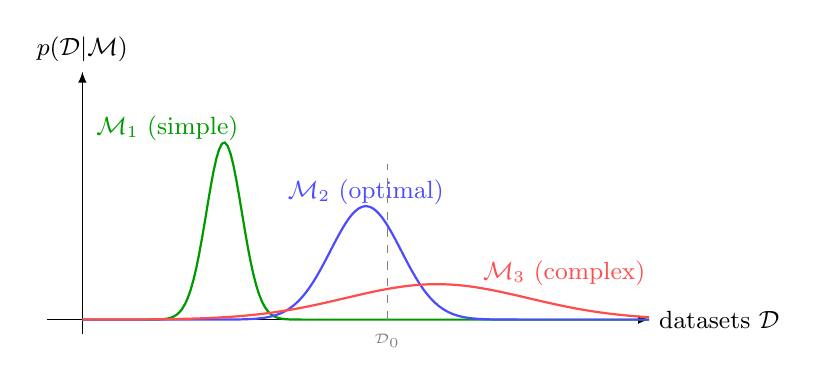
\begin{tikzpicture}[scale=0.9]
    \draw[->] (-0.5,0) -- (8,0) node[right,font=\small] {datasets $\mathcal{D}$};
    \draw[->] (0,-0.2) -- (0,3.5) node[above,font=\small] {$p(\mathcal{D}|\mathcal{M})$};
    % Simple model - narrow
    \draw[green!60!black,thick,domain=0:8,samples=200]
      plot (\x, {2.5*exp(-8*(\x-2)^2)});
    \node[green!60!black,font=\small] at (1.2,2.7) {$\mathcal{M}_1$ (simple)};
    % Intermediate
    \draw[blue!70,thick,domain=0:8,samples=200]
      plot (\x, {1.6*exp(-2*(\x-4)^2)});
    \node[blue!70,font=\small] at (4,1.8) {$\mathcal{M}_2$ (optimal)};
    % Complex model - flat
    \draw[red!70,thick,domain=0:8,samples=200]
      plot (\x, {0.5*exp(-0.3*(\x-5)^2)});
    \node[red!70,font=\small] at (6.8,0.65) {$\mathcal{M}_3$ (complex)};
    % Observed data
    \draw[dashed,gray] (4.3,0) -- (4.3,2.2);
    \node[font=\tiny,gray] at (4.3,-0.3) {$\mathcal{D}_0$};
  \end{tikzpicture}
  \end{center}
  \small
  \begin{itemize}
    \item $\mathcal{M}_1$: too narrow — assigns near-zero probability to $\mathcal{D}_0$.
    \item $\mathcal{M}_3$: too broad — spreads probability mass thin.
    \item $\mathcal{M}_2$: highest evidence at $\mathcal{D}_0$ — best balance.
  \end{itemize}
\end{frame}

\begin{frame}{Bayesian Model Comparison}{Automatic Occam's Razor}
  \begin{exampleblock}{Key Properties of Bayesian Model Selection}
    \begin{enumerate}
      \item \textbf{Automatic Occam's Razor}: complex models are penalized by the ratio of posterior-to-prior volume — no manual regularization needed.
      \item \textbf{No test set required}: hyperparameters can be tuned by maximizing evidence on training data alone.
      \item \textbf{Quantified uncertainty}: predictions are formed as a mixture, acknowledging model uncertainty.
    \end{enumerate}
  \end{exampleblock}

  \begin{itemize}
    \item Avoids overfitting even without cross-validation.
    \item Provides a rigorous framework for comparing models of different structural complexity.
  \end{itemize}
\end{frame}

% =============================================================
\section{The Evidence Framework}
% =============================================================

\subsection{Analytical Evidence for Linear Regression}

\begin{frame}{Evidence Framework}{Log-Evidence for Linear Regression}
  \textbf{Setup}: $t = \w^T\x + \varepsilon$, $\varepsilon \sim \mathcal{N}(0,\beta^{-1})$; prior $p(\w|\alpha) = \mathcal{N}(\Zero,\alpha^{-1}\mathbf{I})$.

  After completing the square and integrating out $\w$:

  \begin{block}{Analytical Log-Evidence}
    \[
      \log p(\t|\X,\alpha,\beta) = \frac{M}{2}\log\alpha + \frac{n}{2}\log\beta - E(\w_{MAP}) - \frac{1}{2}\log|\mathbf{A}| - \frac{n}{2}\log(2\pi)
    \]
    where $\mathbf{A} = \alpha\mathbf{I} + \beta\X^T\X$ is the Hessian and $E(\w_{MAP})$ the MAP residual error.
  \end{block}

  \begin{itemize}
    \item $-E(\w_{MAP})$: data fit — better fit $\to$ higher evidence.
    \item $-\frac{1}{2}\log|\mathbf{A}| + \frac{M}{2}\log\alpha$: Occam penalty — grows with complexity.
    \item As model complexity increases: fit improves but penalty increases.
  \end{itemize}
\end{frame}

\begin{frame}{Evidence Framework}{Optimizing Hyperparameters: $\alpha$ and $\beta$}
  \begin{block}{Evidence Framework}
    Instead of cross-validation, maximize log-evidence w.r.t.\ hyperparameters $\alpha$ (prior precision) and $\beta$ (noise precision).
  \end{block}

  Define the \textbf{effective number of well-determined parameters}:
  \[
    \gamma = \sum_{i=1}^M \frac{\lambda_i}{\lambda_i + \alpha}
  \]
  where $\lambda_i$ are eigenvalues of $\beta\X^T\X$.

  \begin{block}{Optimal Hyperparameters (iterative updates)}
    \[
      \alpha = \frac{\gamma}{\w_{MAP}^T\w_{MAP}}, \qquad \frac{1}{\beta} = \frac{1}{n-\gamma}\sum_{i=1}^n(t_i - \w_{MAP}^T\x_i)^2
    \]
  \end{block}
\end{frame}

\begin{frame}{Evidence Framework}{Interpreting Well-Determined Parameters}
  The quantity $\gamma = \sum_{i=1}^M \frac{\lambda_i}{\lambda_i + \alpha}$ with $0 \le \gamma \le M$:

  \begin{columns}
    \begin{column}{0.47\textwidth}
      \begin{block}{$\lambda_i \gg \alpha$ (data-driven)}
        \begin{itemize}
          \item Contribution to $\gamma \approx 1$
          \item Parameter is \textbf{well-determined} by data
          \item Data dominates the prior
        \end{itemize}
      \end{block}
    \end{column}
    \begin{column}{0.47\textwidth}
      \begin{block}{$\lambda_i \ll \alpha$ (prior-driven)}
        \begin{itemize}
          \item Contribution to $\gamma \approx 0$
          \item Parameter \textbf{shrunk} toward zero
          \item Prior dominates the data
        \end{itemize}
      \end{block}
    \end{column}
  \end{columns}

  \bigskip
  \begin{exampleblock}{Internal Validation}
    The evidence framework measures how much information the data provides vs.\ the prior, and adjusts $\alpha$ and $\beta$ accordingly. This \textbf{eliminates the need for expensive $K$-fold cross-validation}.
  \end{exampleblock}
\end{frame}

% =============================================================
\section{Summary}
% =============================================================

\begin{frame}{Summary}{Probabilistic Learning: Key Results}
  \begin{columns}
    \begin{column}{0.47\textwidth}
      \begin{block}{Decision Theory}
        \begin{itemize}
          \item Optimal classifier: max posterior
          \item Asymmetric costs $\to$ shifted threshold
          \item Reject option for high uncertainty
          \item Regression: predict conditional mean
        \end{itemize}
      \end{block}

      \begin{block}{MLE and MAP}
        \begin{itemize}
          \item MLE: maximize likelihood
          \item Gaussian likelihood $\equiv$ L2 loss
          \item MAP: MLE + prior
          \item Gaussian prior $\equiv$ L2 regularization
        \end{itemize}
      \end{block}
    \end{column}
    \begin{column}{0.47\textwidth}
      \begin{block}{Model Selection}
        \begin{itemize}
          \item Validation: test set, $K$-fold, LOO
          \item AIC: minimizes prediction error
          \item BIC: consistent, more conservative
          \item Bayesian: evidence = automatic Occam
        \end{itemize}
      \end{block}

      \begin{block}{Full Bayesian}
        \begin{itemize}
          \item Posterior $\to$ predictive distribution
          \item Model averaging weights by evidence
          \item Evidence framework: tune $\alpha, \beta$ from data
          \item No external validation needed
        \end{itemize}
      \end{block}
    \end{column}
  \end{columns}
\end{frame}

\begin{frame}{Summary}{Central Message}
  \begin{center}
  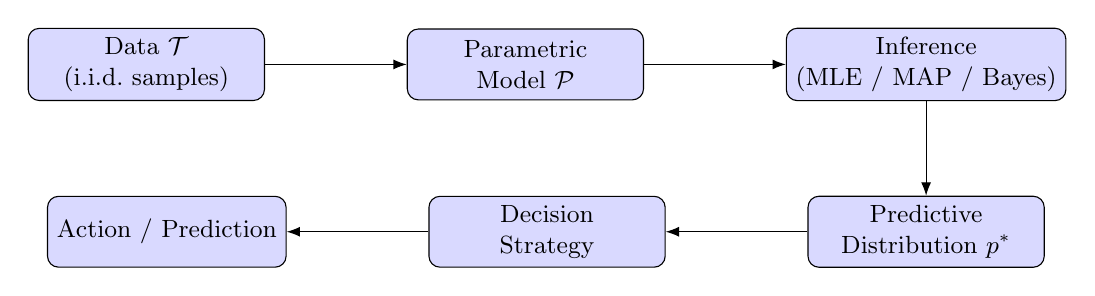
\begin{tikzpicture}[node distance=1.8cm, >=Latex, font=\small,
    box/.style={draw, rounded corners, fill=blue!15, minimum width=3cm, minimum height=0.9cm, align=center}]
    \node[box] (pdata) {Data $\mathcal{T}$\\(i.i.d.\ samples)};
    \node[box, right=of pdata] (model) {Parametric\\Model $\mathcal{P}$};
    \node[box, right=of model] (inf) {Inference\\(MLE / MAP / Bayes)};
    \node[box, below=1.2cm of inf] (pred) {Predictive\\Distribution $p^*$};
    \node[box, left=of pred] (dec) {Decision\\Strategy};
    \node[box, left=of dec] (action) {Action / Prediction};
    \draw[->] (pdata) -- (model);
    \draw[->] (model) -- (inf);
    \draw[->] (inf) -- (pred);
    \draw[->] (pred) -- (dec);
    \draw[->] (dec) -- (action);
  \end{tikzpicture}
  \end{center}

  \bigskip
  \begin{itemize}
    \item \textbf{Model choice} (hypothesis space) encodes inductive bias — unavoidable.
    \item \textbf{Inference} calibrates the model to data — MLE is the simplest approach.
    \item \textbf{Regularization} = prior beliefs on parameters.
    \item \textbf{Model selection} identifies the right complexity level.
    \item \textbf{Bayesian evidence} provides the most principled model comparison.
  \end{itemize}
\end{frame}

\begin{frame}{Summary}{Key Formulas at a Glance}
  \begin{center}
  \begin{tabular}{ll}
    \toprule
    \textbf{Result} & \textbf{Formula / Statement}\\
    \midrule
    Optimal classifier & $h(\x)=\argmax_{k} p(\mathcal{C}_k|\x)$\\
    Optimal regressor & $h^*(\x) = \mathbb{E}[t|\x]$\\
    MLE & $\Vtheta^*_{ML} = \argmax_{\Vtheta} \sum_i \ln p(t_i|\x_i,\Vtheta)$\\
    MAP & $\Vtheta^*_{MAP} = \argmax_{\Vtheta} (l(\Vtheta|\mathcal{T})+\ln p(\Vtheta))$\\
    AIC & $2|\Vtheta| - 2\ln L(\Vtheta_{ML}|\mathcal{T})$\\
    BIC & $|\Vtheta|\ln n - 2\ln L(\Vtheta_{ML}|\mathcal{T})$\\
    Model Evidence & $p(\mathcal{T}|\mathcal{M}) = \int p(\mathcal{T}|\w,\mathcal{M})\,p(\w|\mathcal{M})\,d\w$\\
    Log-Evidence & $\approx \ln p(\mathcal{T}|\w_{MAP},\mathcal{M}) + M\ln\!\frac{\Delta w_{pos}}{\Delta w_{pri}}$\\
    Predictive Dist.\ & $p(t|\x,\mathcal{T}) = \sum_i p(t|\x,\mathcal{M}_i,\mathcal{T})\,p(\mathcal{M}_i|\mathcal{T})$\\
    \bottomrule
  \end{tabular}
  \end{center}
\end{frame}

%\end{document}
